\glsresetall


\chapter{Einleitung}
Die \gls{HDR} Bildgebung ist eines von vielen interessanten Problemen in dem aufstrebenden Forschungsgebiet \textit{Computational Photography}. Bei diesen Bildern handelt es sich um Repräsentationen einer realen Szene, die - im Vergleich zu herkömmlichen Aufnahmen - einen erhöhten Dynamikumfang (Verhältnis zwischen hellstem und dunkelstem Pixel im Bild) besitzen und somit u.a. größere Helligkeitsbereiche darstellen können. Ziel dieser Arbeit ist die Fusion mehrerer Bilder mit verschiedener Belichtungszeit zu einem einzigen Bild mit deutlich vergrößertem Dynamikumfang.
 
\section{Motivation}


Während viele Arbeiten sich nur mit der pixelweisen Fusion der Bilddaten auseinander setzen, schlagen Debevec und Malik \cite{paper} vor, gleichzeitig auch noch die Antwortkurve des Bildaufnahmeprozesses, d.h. der verwendeten Kamera, mitzuschätzen. Diese Antwortkurve ist die kameraspezifische Abbildung, welche aus den Beleuchtungswerten der aufzunehmenden Szene Grau- bzw. Farbwerte erzeugt (siehe \autoref{fig:antwortkurve}).

Dies bietet den klaren Vorteil, die Bildfusion auch ohne vorherige radiometrische Kalibration des Aufnahmeequipments durchführen zu können. Als mathematisches Werkzeug zur Formulierung des Verfahrens dient hierbei ein gemeinsames Energiefunktional, das einen Ähnlichkeits- und einen  Glattheitsterm besitzt. Während der Ähnlichkeitsterm unter Berücksichtigung der mitgeschätzten Antwortkurve die Beziehung zwischen den Einzelaufnahmen und dem gesuchten HDR-Bild herstellt, sorgt der Glattheitsterm für eine hinreichend glatte Antwortkurve, die auch aus radiometrischer Sicht Sinn ergibt.

\begin{figure}
  \begin{center}
    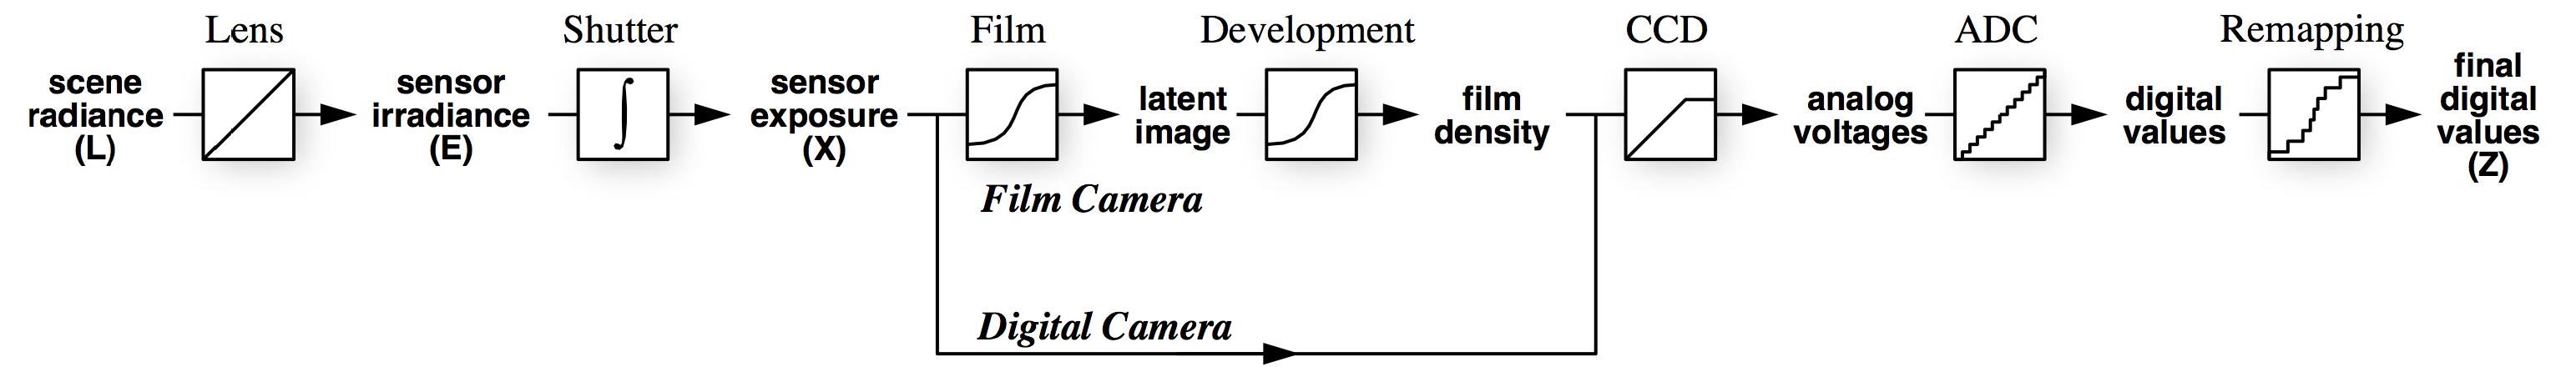
\includegraphics[width=\textwidth]{ImageAquisitionPipeline}
    \caption{\textit{Bildaufnahme-Pipeline} --- Veranschaulichung der zu durchlaufenden Prozesse bei der Aufnahme eines Bildes mit einer Kamera  \cite[S.2]{paper}.}
    \label{fig:antwortkurve}
  \end{center}
\end{figure}

Trotz der allgemeinen Formulierung hat das Verfahren von Debevec und Malik jedoch auch einige Schwachstellen. Zum einen werden weder im Daten- noch im Glattheitsterm robuste Bestrafungsfunktionen verwendet. Diese könnten den Ansatz deutlich robuster unter Fehlmessungen machen. Zum anderen werden keine Beschränkungen gefordert, die die typischerweise gewünschte Monotonie der Antwortkuve explizit erzwingen würden. Monotone Kurven können deshalb nur bei einer hinreichend großen Gewichtung der Glattheit erzielt werden. Schließlich ist das Verfahren auch nicht sonderlich robust gegenüber Rauschen, was insbesondere bei sehr kurz belichteten Bildern Probleme bereiten kann. 

\section{Aufgabenstellung}
Ziel der Arbeit ist es zunächst das Verfahren von Debevec und Malik \cite{paper} als Ausgangsverfahren in einer (dafür sinnvollen und portierbaren) Programmiersprache zu implementieren.

Diese Implementierung soll anschließend sukzessive um eine Monotonie-Beschränkung (siehe \autoref{sec:monotonie}), einen räumlichen Glattheitsterm (siehe \autoref{sec:raeumlich}) und robuste Bestrafungsfunktionen (siehe \autoref{sec:robustheit}) erweitert werden.

\begin{figure}[H]
  \begin{center}
      \begin{overpic}[width=0.48\textwidth]{teezer/E_noise_no_robustness}
                \put(-0,0){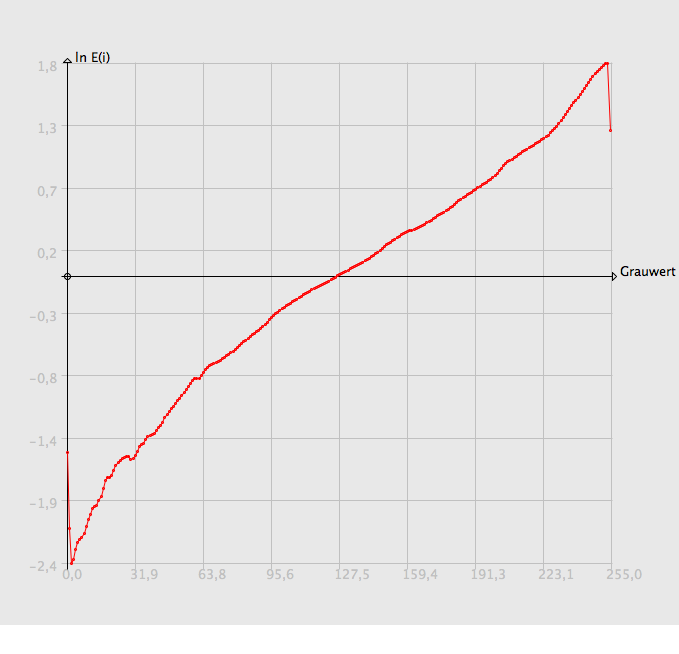
\includegraphics[width=2cm]{teezer/g_noise_no_robustness}}
        \end{overpic}
        \hfill
        \begin{overpic}[width=0.48\textwidth]{teezer/E_noise_robustness_raum}
            \put(-0,0){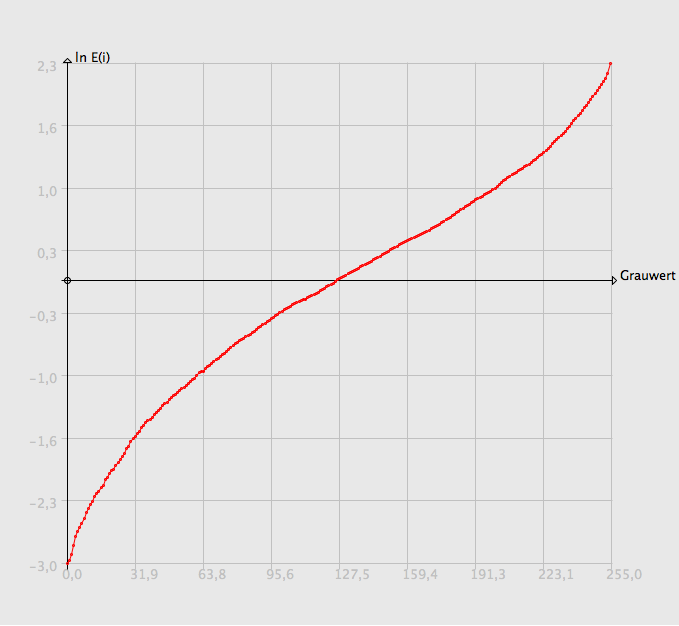
\includegraphics[width=2cm]{teezer/g_noise_robustness_raum}}
        \end{overpic}
    \caption{\textit{Antwortkurven (incl. zugehörigem HDR-Bild)} --- Das HDR-Bild wurde mittels lokalem Reinhard-Tone-Mapper (siehe \autoref{subsec:ToneMapping}) erstellt. \textbf{links}: Ohne robuste Bestrafungsterme. \textbf{rechts}: Mit robusten Bestrafungstermen und räumlicher Glattheitsforderung.}
    \label{fig:teezer}
  \end{center}
\end{figure}


Neben der Modellierung und Implementierung der einzelnen Erweiterungen soll auch eine geeignete visuelle Evaluation der Ergebnisse erfolgen. Hierzu sollen \gls{Tone-Mapping}-Verfahren (siehe \autoref{subsec:ToneMapping}) aus bereits existierender Forschung verwendet werden. 


\section{Gliederung}
In \autoref{chap:hdr} werden zunächst die Grundlagen der \gls{HDR}-Bilder vermittelt. Dabei wird auf die physikalischen, historischen und anwendungsorientierten Eigenschaften von \gls{HDR}-Bildern eingegangen. Im anschließenden \autoref{chap:references} werden verwandte Arbeiten zum Thema \gls{HDR} zusammengefasst sowie existierende Implementierungen des Ansatzes von Debevec und Malik vorgestellt.

Die zu Grunde liegende Vorgehensweise von Debevec und Malik wird im nachfolgenden \autoref{chap:algo} beschrieben. Außerdem werden die existierenden Schwachstellen des bisherigen Ansatzes dargestellt und erläutert. Darauf basierend wird dann im \autoref{chap:maths} mathematisch umgesetzt und diskutiert. Außerdem werden die Erweiterungen des Algorithmus beschrieben und formal spezifiziert.

Im \autoref{chap:impl} wird die Herangehensweise an die Problemstellung aus Sicht der Entwicklung beschrieben. Es werden Anforderungen an die Software formuliert, der Prototyp vorgestellt und die Architektur der Implementierung beschrieben. Abschließend wird die Verwendung der Software erläutert.

Das \autoref{chap:results} stellt die Resultate und Einflüsse der unterschiedlichen Erweiterungen vor. Die Ergebnisse werden mit dem Standard-Ansatz verglichen und es folgt eine Analyse der Resultate.
Das \autoref{chap:zusfas} rundet die vorliegende Arbeit mit einer Zusammenfassung der Ergebnisse und Ausblicken ab. 
